\section{Xem xét thuật toán tính toán toạ độ mục tiêu khác}

\subsection{Tổng quan}
Đề tài tập trung xây dựng các thuật toán nhằm tính toán toạ độ địa lý của mục tiêu (kinh độ, vĩ độ, cao độ) dựa trên dữ liệu đầu vào gồm:
\begin{itemize}
    \item Toạ độ GPS của người quan sát $(\varphi_0, \lambda_0, h_0)$.
    \item Góc ngắm \textit{azimuth} và \textit{elevation} thu được từ cảm biến IMU/la bàn.
    \item Khoảng cách đến mục tiêu $d$ thu được từ cảm biến laser rangefinder.
\end{itemize}

Hai hướng tiếp cận chính được xem xét:
\begin{enumerate}
    \item \textbf{Thuật toán Geometric (ECEF$\rightarrow$ENU)}: chuyển toạ độ người quan sát sang hệ toạ độ địa tâm (ECEF), tạo vectơ hướng trong hệ ENU, quay về ECEF, cộng vectơ dịch chuyển và chuyển ngược sang hệ toạ độ địa lý. Phương pháp này chính xác trên phạm vi toàn cầu. Đây là thuật toán nhóm lựa chọn, đã được thực hiện.
    \item \textbf{Thuật toán Flat-Earth (cải tiến)}: coi vùng xung quanh người quan sát là mặt phẳng tiếp tuyến với Trái Đất, chuyển đổi khoảng cách theo phương Đông - Bắc - Lên, sau đó quy đổi về độ vĩ và độ kinh. Phương pháp này nhanh, nhẹ, đủ chính xác cho phạm vi vài km. 
\end{enumerate}

\subsection{Ký hiệu và hằng số}
\begin{itemize}
    \item Bán trục lớn $a = 6{,}378{,}137.0$ m.
    \item Độ dẹt $f = 1/298.257223563$.
    \item Độ lệch tâm $e^2 = f(2-f)$.
    \item Vĩ độ, kinh độ người quan sát: $\varphi_0$, $\lambda_0$ (độ).
    \item Góc azimuth $A$, góc elevation $el$ (độ).
    \item Khoảng cách nghiêng đến mục tiêu $d$ (m).
\end{itemize}

\subsection{Thuật toán Flat-Earth (cải tiến)}
Giả sử các giá trị góc được chuyển sang radian: 
$\alpha = A \cdot \pi/180$, $\beta = el \cdot \pi/180$.

\subsubsection{Bước 1: Phân tách khoảng cách theo phương ngang và đứng}
\[
    d_h = d\cos\beta, \quad U = d\sin\beta
\] 

\subsubsection{Bước 2: Toạ độ ENU của mục tiêu so với người quan sát}
\[
    E = d_h \sin\alpha, \quad N = d_h \cos\alpha
\]

\subsubsection{Bước 3: Bán kính cong tại vĩ độ trung bình $\varphi_m$}

Đây là bước quan trọng nhất của thuật toán. Tên gọi "Flat-Earth" (Trái Đất phẳng) là một tên gọi sai lầm. Một mô hình Trái Đất phẳng thực sự sẽ sử dụng định lý Pitago đơn giản và giả định một Trái Đất hình cầu.\\

Thuật toán này tinh vi hơn nhiều. Việc nó sử dụng các công thức cho $M(\varphi_m)$ và $N_p(\varphi_m)$ cho thấy nó không phải là mô hình Trái Đất phẳng, mà là một mô hình Xấp xỉ Ellipsoid Cục bộ (Local Ellipsoidal Approximation). Tên gọi "cải tiến" (improved) chính là để chỉ điều này.\\

Thuật toán này không giả định Trái Đất phẳng; nó giả định mặt phẳng tiếp tuyến tại vĩ độ trung bình $\varphi_m$ là một xấp xỉ tốt và sử dụng các bán kính cong của ellipsoid tại điểm đó để tuyến tính hóa phép chuyển đổi từ mét sang độ.

\[
\begin{aligned}
    M(\varphi_m) &= \frac{a(1 - e^2)}{(1 - e^2 \sin^2 \varphi_m)^{3/2}}, \\
    N_p(\varphi_m) &= \frac{a}{\sqrt{1 - e^2 \sin^2 \varphi_m}}.
\end{aligned}
\]

\begin{itemize}
    \item Giải thích $M(\varphi_m)$ (Bán kính Cong Kinh tuyến): Đây là bán kính của đường cong theo hướng Bắc-Nam (dọc theo một kinh tuyến). Công thức $M(\varphi_{m})=\frac{a(1-e^{2})}{(1-e^{2}sin^{2}\varphi_{m})^{3/2}}$ là công thức trắc địa tiêu chuẩn cho bán kính này.14 Nó được sử dụng để chuyển đổi khoảng cách $N$ (Bắc).
    \item Giải thích $N_p(\varphi_m)$ (Bán kính Cong Thẳng đứng): Đây là bán kính của đường cong theo hướng Đông-Tây (vuông góc với kinh tuyến). Công thức $N_{p}(\varphi_{m})=\frac{a}{\sqrt{1-e^{2}sin^{2}\varphi_{m}}}$ là công thức trắc địa tiêu chuẩn.14 Nó được sử dụng như một phần của phép chuyển đổi khoảng cách $E$ (Đông).

\end{itemize}



\subsubsection{Bước 4: Quy đổi từ ENU sang thay đổi toạ độ địa lý}
Bước này áp dụng công thức cơ bản của cung tròn (chiều dài cung = bán kính $\times$ góc [rad]) để tìm sự thay đổi góc từ các khoảng cách $N$ và $E$.
\[
\begin{aligned}
    \Delta\varphi &= \frac{N}{M}, \\
    \Delta\lambda &= \frac{E}{N_p \cos\varphi_m}.
\end{aligned}
\]
\begin{itemize}
    \item Giải thích $\Delta\varphi = N / M$:
Phép chuyển đổi vĩ độ rất đơn giản. Sự thay đổi góc vĩ độ (radian) $\Delta\varphi$ là chiều dài cung (khoảng cách Bắc $N$) chia cho bán kính của đường cong Bắc-Nam ($M$).
    \item Giải thích $\Delta\lambda = E / (N_{p} \cos \varphi_{m})$:
Phép chuyển đổi kinh độ tinh vi hơn. Một sai lầm phổ biến là chia $E$ cho $N_p$. Tuy nhiên, bán kính của một chuyển động Đông-Tây không phải là $N_p$ (là bán kính thẳng đứng). Bán kính của vòng tròn mà một người đi theo khi di chuyển về phía Đông là bán kính của vòng tròn vĩ tuyến (parallel of latitude) tại vĩ độ đó.
Như 15 giải thích, các vòng tròn vĩ tuyến co lại từ xích đạo (nơi bán kính của chúng là $N_p$) về các cực (nơi bán kính của chúng bằng 0), theo hàm cosin của vĩ độ.
Do đó, bán kính của vòng tròn vĩ tuyến tại $\varphi_m$ là $N_p(\varphi_m) \cdot \cos(\varphi_m)$.
Vì vậy, sự thay đổi góc kinh độ (radian) $\Delta\lambda$ là chiều dài cung (khoảng cách Đông $E$) chia cho bán kính của vòng tròn vĩ tuyến ($N_p \cos \varphi_m$). Thuật toán trong 1 đã thực hiện điều này một cách chính xác.

\end{itemize}

\subsubsection{Bước 5: Toạ độ mục tiêu}
\[
\begin{aligned}
    \varphi_1 &= \varphi_0 + \Delta\varphi \cdot \frac{180}{\pi},\\
    \lambda_1 &= \lambda_0 + \Delta\lambda \cdot \frac{180}{\pi},\\
    h_1 &= h_0 + U.
\end{aligned}
\]
Các tọa độ ngang đơn giản là phép cộng đại số. Tuy nhiên, phép tính độ cao, $h_1 = h_0 + U$ 1, là một sự đơn giản hóa quan trọng sẽ được phân tích trong phần tiếp theo. Phương pháp này cho độ chính xác rất cao trong phạm vi ngắn (sai số $\approx$ mm với khoảng cách dưới 500~m), nhưng sai lệch tăng theo khoảng cách do giả thiết mặt phẳng tiếp tuyến.
\subsection{Ví dụ minh hoạ (chi tiết) — Flat-Earth (improved)}
Trong phần này ta làm một ví dụ số \textbf{từng bước} theo đúng các công thức của phương pháp Flat-Earth (improved).

\subsubsection*{Dữ liệu đầu vào}
\[
\begin{aligned}
&\varphi_0 = 10.000000^\circ,\quad \lambda_0 = 106.000000^\circ,\quad h_0 = 10.0\ \mathrm{m},\\
&\text{Azimuth } A = 63.232668^\circ,\quad \text{Elevation } el = 2.330536^\circ,\quad d = 245.799463\ \mathrm{m}.
\end{aligned}
\]

\subsubsection*{Bước 1: Quy đổi góc sang radian}
\[
\begin{aligned}
\alpha &= A\cdot\frac{\pi}{180} = 63.232668^\circ\cdot\frac{\pi}{180} \approx 1.103997240\ \text{rad},\\[4pt]
\beta &= el\cdot\frac{\pi}{180} = 2.330536^\circ\cdot\frac{\pi}{180} \approx 0.040673593\ \text{rad}.
\end{aligned}
\]

\subsubsection*{Bước 2: Tách khoảng cách thành thành phần ngang và đứng}
\[
\begin{aligned}
d_h &= d\cos\beta = 245.799463\cdot\cos(0.040673593) \approx 245.5961536172\ \mathrm{m},\\[4pt]
U   &= d\sin\beta = 245.799463\cdot\sin(0.040673593) \approx 9.9952658558\ \mathrm{m}.
\end{aligned}
\]

\subsubsection*{Bước 3: Tính vector ENU (East, North, Up)}
\[
\begin{aligned}
E &= d_h \sin\alpha \approx 245.5961536172\cdot\sin(1.103997240) \approx 219.27874458780065\ \mathrm{m},\\[4pt]
N &= d_h \cos\alpha \approx 245.5961536172\cdot\cos(1.103997240) \approx 110.60878285000351\ \mathrm{m},\\[4pt]
U &= 9.995265855755704\ \mathrm{m}\quad(\text{như trên}).
\end{aligned}
\]

\subsubsection*{Bước 4: Tính bán kính cong tại vĩ độ trung bình}
Vì khoảng cách nhỏ, ta chọn vĩ độ trung bình \(\varphi_m \approx \varphi_0\). Dùng hằng số WGS-84:
\[
a = 6\,378\,137.0\ \mathrm{m},\qquad f = \frac{1}{298.257223563},\qquad e^2 = f(2-f).
\]
Tính:
\[
\varphi_m = \varphi_0\cdot\frac{\pi}{180} = 10^\circ\cdot\frac{\pi}{180} \approx 0.174532925199433\ \text{rad}.
\]
\[
\begin{aligned}
M(\varphi_m) &= \frac{a(1-e^2)}{(1 - e^2\sin^2\varphi_m)^{3/2}}
\approx 6\,337\,358.121554948\ \mathrm{m},\\[4pt]
N_p(\varphi_m) &= \frac{a}{\sqrt{1 - e^2\sin^2\varphi_m}}
\approx 6\,378\,780.843661353\ \mathrm{m}.
\end{aligned}
\]

\subsubsection*{Bước 5: Tính \(\Delta\varphi, \Delta\lambda\) (rad) và đổi sang độ}
\[
\begin{aligned}
\Delta\varphi &= \frac{N}{M} = \frac{110.60878285000351}{6\,337\,358.121554948}
\approx 1.745345311539129\times 10^{-5}\ \text{rad},\\[6pt]
\Delta\lambda &= \frac{E}{N_p\cos\varphi_m}
= \frac{219.27874458780065}{6\,378\,780.843661353\cdot\cos(0.174532925199433)}\\
&\qquad\approx 3.490658765877035\times 10^{-5}\ \text{rad}.
\end{aligned}
\]

Đổi về độ:
\[
\begin{aligned}
\Delta\varphi_{\text{deg}} &= \Delta\varphi\cdot\frac{180}{\pi}\approx 0.0010000092014413793^\circ,\\[4pt]
\Delta\lambda_{\text{deg}} &= \Delta\lambda\cdot\frac{180}{\pi}\approx 0.0020000001500509864^\circ.
\end{aligned}
\]

\subsubsection*{Bước 6: Tọa độ mục tiêu (theo Flat-Earth improved)}
\[
\begin{aligned}
\varphi_1 &= \varphi_0 + \Delta\varphi_{\text{deg}}
= 10.000000^\circ + 0.0010000092014413793^\circ \\
&\qquad\approx \mathbf{10.001000009201441^\circ},\\[6pt]
\lambda_1 &= \lambda_0 + \Delta\lambda_{\text{deg}}
= 106.000000^\circ + 0.0020000001500509864^\circ \\
&\qquad\approx \mathbf{106.00200000015005^\circ},\\[6pt]
h_1 &= h_0 + U = 10.0 + 9.995265855755704 \approx \mathbf{19.995265855755704\ \mathrm{m}}.
\end{aligned}
\]



\subsection{Kết quả thử nghiệm và so sánh}
Với bộ dữ liệu thử nghiệm:
\[
\begin{aligned}
    \varphi_0 &= 10.000000^\circ, \quad \lambda_0 = 106.000000^\circ, \quad h_0 = 10.0~\mathrm{m},\\
    A &= 63.232668^\circ, \quad el = 2.330536^\circ, \quad d = 245.799463~\mathrm{m}.
\end{aligned}
\]

Kết quả tính toán:

\begin{table}[H]
\centering
\caption{So sánh kết quả giữa hai thuật toán}
\begin{tabular}{lccc}
\hline
\textbf{Thuật toán} & $\varphi_1$ (deg) & $\lambda_1$ (deg) & $h_1$ (m) \\
\hline
Flat-Earth (cải tiến) & 10.0010000092 & 106.00200000015 & 19.9953 \\
Geometric (ECEF) & 10.0010000000 & 106.0020000000 & 20.0000 \\
\hline
Sai lệch & $\approx$ 0.001 mm & $\approx$ 0.0001 mm & $\approx$ 4.7 mm \\
\hline
\end{tabular}
\end{table}

Sai số giữa hai thuật toán là rất nhỏ (ở mức milimét), chứng tỏ phương pháp Flat-Earth hoàn toàn phù hợp cho phạm vi vài trăm mét.

\subsection{Phân tích sai số và lựa chọn thuật toán}
Phân tích Bảng 7 cho thấy một sự không tương xứng rõ rệt: chênh lệch ngang (vĩ độ, kinh độ) ở mức sub-milimét, trong khi chênh lệch dọc (cao độ) lớn hơn hàng nghìn lần, ở mức 4.7 mm.

Sự chênh lệch này không phải là ngẫu nhiên. Nó là kết quả trực tiếp của sự đơn giản hóa trong Bước 5 của thuật toán Flat-Earth.
\begin{itemize}
    \item Như đã phân tích trong Phần 3, các bước tính toán ngang (E, N) của thuật toán Flat-Earth là các xấp xỉ ellipsoid cục bộ tinh vi (sử dụng $M$ và $N_p \cos \varphi_m$). Đây là lý do tại sao chúng gần như hoàn toàn khớp với kết quả của thuật toán Geometric (sai số 0.001 mm).
    \item Tuy nhiên, bước tính toán dọc là $h_1 = h_0 + U$. $U$ là thành phần "Lên" (Up) so với mặt phẳng tiếp tuyến của người quan sát.
    \item Do độ cong của Trái Đất, vector "Up" (vuông góc với ellipsoid) tại vị trí mục tiêu (cách 245m) không song song với vector "Up" tại vị trí người quan sát.
    \item Thuật toán Geometric (ECEF) tự động tính toán điều này. Bằng cách giải $(X_1, Y_1, Z_1)$ trong không gian 3D và sau đó giải $h_1$ từ vị trí đó (Bước 2.5), nó tìm thấy độ cao của mục tiêu so với bề mặt ellipsoid bên dưới nó.
    \item Do đó, chênh lệch 4.7 mm chính là sai số hình học—độ "rơi" (drop) của đường chân trời—do việc bỏ qua độ cong của Trái Đất trong phép tính độ cao trên khoảng cách 245m. Mặc dù nhỏ, nó cho thấy điểm yếu lý thuyết của mô hình Flat-Earth: nó xử lý độ cao một cách "phẳng" trong khi xử lý vị trí ngang một cách "cong" (ellipsoidal).
\end{itemize}

Từ đó có thể đưa ra so sánh cơ bản:

\begin{itemize}
    \item Thuật toán Flat-Earth (cải tiến): Như được trình bày trong , toàn bộ thuật toán bao gồm một số lượng cố định các phép toán đại số và lượng giác (sin, cos, sqrt, pow). Không có vòng lặp. Chi phí tính toán của nó thấp và, quan trọng hơn, có thể dự đoán được (deterministic).
    \item Thuật toán Geometric (ECEF ENU):
Thuật toán này bao gồm tất cả các phép tính của thuật toán Flat-Earth (trong các bước LLA $\rightarrow$ ECEF và AER $\rightarrow$ ENU) cộng thêm điểm nghẽn tính toán (ECEF $\rightarrow$ LLA).
Bước ECEF $\rightarrow$ LLA  đòi hỏi một giải pháp lặp (như Newton-Raphson) hoặc giải một phương trình bậc 4 phức tạp.
Do đó, thuật toán Flat-Earth "nhanh hơn" không chỉ vì nó có ít phép toán hơn, mà vì nó tránh được bài toán nghịch đảo (inverse problem) vốn đòi hỏi phép lặp. Phép cộng đại số đơn giản trong Bước 5 của nó ($\varphi_1 = \varphi_0 + \Delta\varphi$) thực chất là một xấp xỉ tuyến tính, một bước của bài toán nghịch đảo, thay thế một vòng lặp có chi phí thay đổi bằng một phép toán có chi phí cố định và thấp.

\end{itemize}

Vậy, có thể thấy:

\begin{itemize}
    \item \textbf{Nguồn sai số:} do giả thiết mặt phẳng, độ cong ellipsoid bị bỏ qua, sai số cảm biến (GPS, la bàn, IMU, laser).
    \item \textbf{Khoảng cách ngắn ($<1$~km):} sai số của Flat-Earth nhỏ hơn $0.1$~m.
    \item \textbf{Khoảng cách trung bình (1--5~km):} sai số tăng lên vài mét, có thể chấp nhận cho UAV hoặc hệ quan sát tầm gần.
    \item \textbf{Khoảng cách lớn ($>10$~km):} cần dùng Geometric để đảm bảo chính xác.
\end{itemize}

\subsection{Đánh giá và biểu diễn kết quả}
Nhóm tiến hành so sánh theo các tiêu chí:
\begin{itemize}
    \item \textbf{Sai số vị trí (m)} giữa hai thuật toán.
    \item \textbf{Ảnh hưởng của nhiễu} trong các góc đo và khoảng cách.
    \item \textbf{Hiệu năng tính toán} (thời gian xử lý).
\end{itemize}

\begin{figure}[H]
    \centering
    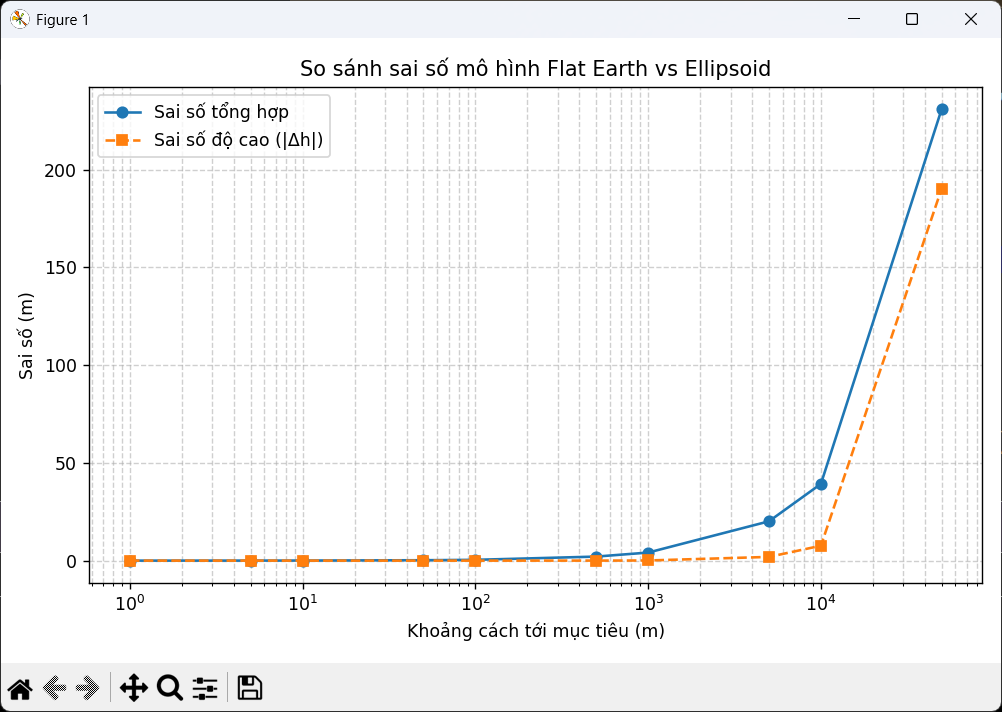
\includegraphics[scale=0.5]
    {Images/FlatEarth}
    \vspace{0.4cm} 
    \caption{Đồ thị biểu diễn kết quả so sánh sai số giữa 2 mô hình}
\end{figure}

\subsection{Kết luận}
\begin{itemize}
    \item Thuật toán \textbf{Flat-Earth (cải tiến)} đạt độ chính xác tương đương Geometric trong phạm vi vài km, đồng thời tính toán nhanh và đơn giản, phù hợp cho hệ thống nhúng hoặc UAV.
    \item Thuật toán \textbf{Geometric (ECEF$\rightarrow$ENU)} đảm bảo tính chính xác toàn cầu, thích hợp cho ứng dụng đo xa hoặc yêu cầu sai số ở mức cm.
\end{itemize}
